%
% $XORP: xorp/docs/fea/fea.tex,v 1.6 2003/06/09 20:02:20 pavlin Exp $
%

\documentclass[11pt]{article}

%\usepackage[dvips]{changebar}

\usepackage{subfigure}
\usepackage{fullpage}
\usepackage{setspace}
\usepackage{times}
\usepackage{latexsym}
\usepackage{psfig}
\usepackage{graphicx}
\usepackage{xspace}
\usepackage{color}
\usepackage{amsmath}
%\usepackage[dvipdf]{graphics}
%\usepackage[dvips]{graphicx}
%\usepackage{xorp}

\definecolor{gray}{rgb}{0.5,0.5,0.5}
\newcommand{\etc}{\emph{etc.}\xspace}
\newcommand{\ie}{\emph{i.e.,}\xspace}
\newcommand{\eg}{\emph{e.g.,}\xspace}
%\newcommand{\comment}[1]{{\color{gray}[\textsf{#1}]}}
\newcommand{\comment}[1]{}

% Changebar stuff
% \newenvironment{colorcode}{\color{blue}}{}
% \renewcommand{\cbstart}{\begin{colorcode}}
% \renewcommand{\cbend}{\end{colorcode}}

% \pagestyle{empty}

\begin{document}

\title{XORP Forwarding Engine Abstraction \\
\vspace{1ex}
Version 0.4}
\author{ XORP Project					\\
	 International Computer Science Institute	\\
	 Berkeley, CA 94704, USA			\\
	 {\it feedback@xorp.org}
}
\date{August 28, 2003}

\maketitle

\thispagestyle{empty}


%%%%%%%%%%%%%%%%%%%%%%%%%%%%%%%%%%%%%%%%%%%%%%%%%%%%%%%%%%%%%%%%%%%%%%%
\section{Introduction}
\label{sec:introduction}

The role of the Forwarding Engine Abstraction (FEA) in XORP is to
provide a uniform interface to the underlying forwarding engine.  It
shields XORP processes from concerns over variations between
platforms.  As a result, XORP processes need not be concerned whether
the router is comprised of a single machine, or cluster of machines;
or whether the network interfaces are simple, like a PCI Ethernet
adapter, or are smart and have processing resources, like an Intel IXP
cards.

The FEA performs three distinct roles: \emph{interface management},
\emph{forwarding table management}, and \emph{interface specific
packet I/O}.  Those are described briefly in
Section~\ref{sec:introduction:interface_management},
Section~\ref{sec:introduction:forwarding_table_management},
and Section~\ref{sec:introduction:interface_specific_packet_io}
respectively.
Section~\ref{sec:design_and_implementation} presents
the design and implementation of the FEA components.
FEA status summary is in Section~\ref{sec:status}.

Note that the multicast-specific tasks are handled by the Multicast
Forwarding Engine Abstraction (MFEA) which is logically separate from
the FEA, but typically would be part of the FEA process.
For information about the MFEA architecture, see \cite{xorp:mfea}.

%%%%%%%%%%%%%%%%%%%%%%%%%%%%%%%%%%%%%%%%%%%
\subsection{Interface Management}
\label{sec:introduction:interface_management}

In the normal course of interaction, the RouterManager process is the
principal source of interface configuration requests to the FEA.  The
RouterManager constructs the interface configuration from the router
configuration files and the input it receives at the command line.
The type of requests the RouterManager sends to the FEA are to enable
interfaces, create virtual interfaces, set interface MTU's, and so
forth.  The FEA interprets and executes these requests in a manner
appropriate for the underlying forwarding plane.

Processes can register with the FEA to be notified of changes in
interface configuration.  The registered processes are notified of
changes, and may query the FEA on the receipt of an update notification
to determine the change that occurred.  These notifications are
primarily of interest to routing protocols since these need to know
what the state of each interface is at a given time.

\begin{figure}[htbp]
  \begin{center}
    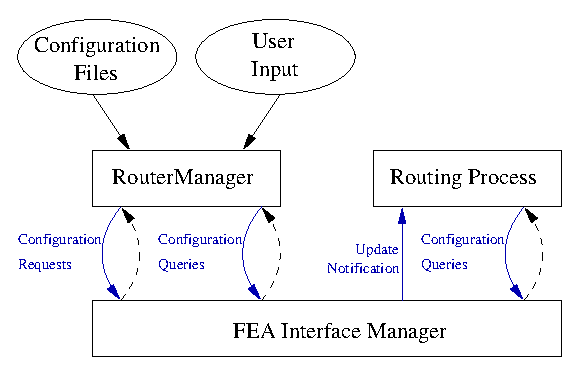
\includegraphics[width=0.80\textwidth]{figs/ifmgmt}
    \caption{FEA Interface Management interaction with other XORP processes}
    \label{fig:ifmgmt}
  \end{center}
\end{figure}

Both of the above interactions are depicted in Figure~\ref{fig:ifmgmt}.

%%%%%%%%%%%%%%%%%%%%%%%%%%%%%%%%%%%%%%%%%%%
\subsection{Forwarding Table Management}
\label{sec:introduction:forwarding_table_management}

The FEA primarily receives forwarding table configuration information from the
RIB process.  The RIB arbitrates between the routes proposed by the
different routing processes, and propagates the results into the FEA's
forwarding table interface.  The FEA accepts requests to insert and
remove routing entries and propagates the necessary changes into the
forwarding plane.  The FEA also supports queries on the current
contents of the forwarding table.

%%%%%%%%%%%%%%%%%%%%%%%%%%%%%%%%%%%%%%%%%%%
\subsection{Interface Specific Packet I/O}
\label{sec:introduction:interface_specific_packet_io}

Routing protocols, such as OSPF, need to be able to send and receive
packets on specific interfaces in the forwarding plane in order to
exchange routing information and to determine the liveness of
connected paths.  Since the forwarding plane may be distributed across
multiple machines, these routing protocols delegate the I/O operations
on these packets to the FEA.  The FEA supports sending and receiving
raw and UDP~\footnote{Currently (August 2003), UDP support
is not present.}  packets on specific interfaces.  The transmission of
packets through the FEA is straightforward, the routing process simply
hands the FEA a packet and indicates which interface it should be sent
on.  The reception of packets is handled through a register-notify
interface where the routing process registers which types of packets
on which interfaces it is interested.

%%%%%%%%%%%%%%%%%%%%%%%%%%%%%%%%%%%%%%%%%%%%%%%%%%%%%%%%%%%%%%%%%%%%%%%
\section{Design and Implementation}
\label{sec:design_and_implementation}

%%%%%%%%%%%%%%%%%%%%%%%%%%%%%%%%%%%%%%%%%%%
\subsection{Overview}

The FEA fulfills three discrete roles: Interface Management, Forwarding
Table Management, and Interface Specific Packet I/O.  The Interface
Management and Forwarding Table Management roles follow a similar
design pattern since both relate to the setting and getting of
configuration state.  The Interface Specific Packet I/O has little in
common with the other two roles.  

The Interface Management and Forwarding Table Management roles use
transactions for setting configuration state.  The transactions are a
collection of grouped operations that are queued until committed or
aborted.  Transactions provide atomic updates to the forwarding plane,
which has the virtue of ensuring a consistent state at any particular
instant of time.  In addition, forwarding plane updates may incur per
update costs, and grouping operations may help to reduce
these. Queries of the configuration state happen on the immediate
state, and are independent of any transactions that are in progress.

The FEA, as with other XORP processes, uses the XRL mechanism for
inter-process communication and each role of the FEA is represented by
a distinct XRL interface.  The Interface Management and Interface
Specific Packet I/O roles support the notion of clients that notified
when event occur and client processes are expected to implement known
interfaces.  The FEA XRL and FEA XRL client interfaces are shown in
Table~\ref{tbl:xifs}.

\begin{table}[h]
\begin{center}
\begin{tabular}{|l|l|l|}\hline
Role & XRL Interface file & Client XRL Interface\\ \hline\hline
Interface Management 		& fea\_ifmgr.xif	& fea\_ifmgr\_client.xif\\
Forwarding Table Management	& fti.xif 		& \\
Interface Specific Packet I/O	& fea\_rawpkt.xif 	& fea\_rawpkt\_client.xif\\ \hline
\end{tabular}
\caption{FEA XRL Interfaces (defined in {\tt \$XORP/xrl/target/fea.tgt})}
\label{tbl:xifs}
\end{center}
\end{table}

The XRL handling code is found in {\tt
\$XORP/fea/xrl\_target.\{hh,cc\}}.  Each XRL interface is handled by
an XRL-aware helper class.  The helper class understands the semantics
of the implementation, and maps errors and responses to the appropriate
XRL forms.  The helper classes and their relations to the interfaces
are depicted in Figure~\ref{fig:xrl_ifs}.

\clearpage
\begin{figure}[htbp]
  \begin{center}
    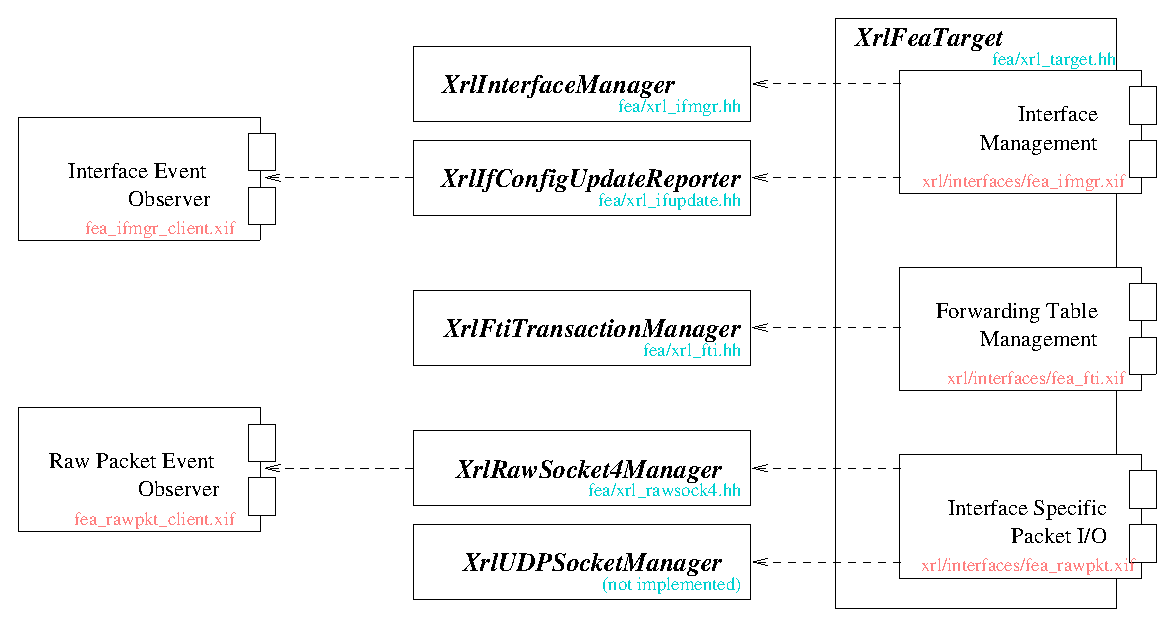
\includegraphics[angle=90,height=0.90\textheight]{figs/xrl_ifs}
    \caption{XRL Interfaces in relation to FEA classes}
    \label{fig:xrl_ifs}
  \end{center}
\end{figure}
\clearpage


%%%%%%%%%%%%%%%%%%%%%%%%%%%%%%%%%%%%%%%%%%%
\subsection{Interface Management}

To succinctly explain the interface management classes and how they
interact we first describe the representation of interface
configuration state.  Interface configuration state is held within
{\tt IfTree} class.  The {\tt IfTree} structure is used and
manipulated by all of the the interface management classes.  The {\tt
IfTree} class is a container of interface state information organized
in a hierarchy:

%% This needs re-presenting - it looks crufty
\begin{description}
\item [\tt IfTree] contains:
  \begin{description}
  \item [\tt IfTreeInterface] physical interface representation, contains:
    \begin{description}
    \item [\tt IfTreeVif] virtual (logical) interface representation, contains:
      \begin{description}
      \item [\tt IfTreeAddr4] Interface IPv4 address and related attributes.
      \item [\tt IfTreeAddr6] Interface IPv6 address and related attributes.
      \end{description}
    \end{description}
  \end{description}
\end{description}

Each item in the IfTree hierarchy is derived from {\tt IfTreeItem}.
{\tt IfTreeItem} is a base class to track the state of a configurable
item. Items may be in one of four states: {\tt CREATED}, {\tt
DELETED}, {\tt CHANGED}, {\tt NO\_CHANGE}.  For example, if an
item is added to the tree it will be in the {\tt CREATED} state.  The
{IfTreeItem::finalize\_state()} method places the item in the {\tt
NO\_CHANGE} state and items marked as {\tt DELETED} are actually
removed at this time.  

The state labeling associated with {\tt IfTreeItem} adds a small
degree of complexity to the {\tt IfTree} classes. However, it allows
for one entity to manipulate an interface configuration tree and pass
it to another entity which can immediately determine the changes from
the state labels.

The interface management functionality of the FEA is represented by
three interacting classes: {\tt IfConfig}, {\tt InterfaceManager},
{\tt InterfaceTransactionManager}.  The interaction of these classes
is managed by the {\tt XrlInterfaceManager}, which takes external XRL
requests and maps them onto the appropriate operations.  The
interactions between these classes and related classes are shown in
Figure~\ref{fig:ifi}. The {\tt XrlInterfaceManager} is sufficiently
aware of the semantics of the operations to pass back human parseable
error messages when operations fail.

The {\tt IfConfig} class is an interface configurator, and contains
plug-ins for each supported forwarding plane architecture to
access, set, or monitor the interface-related information.
The functionality of the {\tt IfConfig} is conceptually simple: it can
push-down an {\tt IfTree} to the forwarding plane or pull-up the live
configuration state from the forwarding plane as an {\tt IfTree}.

The {\tt InterfaceManager} class contains the {\tt IfTree}
representing the live configuration, and a reference to the {\tt
IfConfig} that should be used to perform the configuration.  The {\tt
InterfaceTransactionManager} class holds and dispatches transactions.
Each operation within a transaction operates on an item within a {\tt
IfTree} structure.  Each transaction operates on a copy of the live
{\tt IfTree} and when the commit is made, this structure is pushed
down into the {\tt IfConfig}.

The process of configuration is asynchronous, and two phase.  Errors
can occur whilst a transaction is being committed and operating on an
{\tt Iftree} (\eg because of a bad operation within a transaction), and
errors can occur when the configuration is pushed down to the
forwarding plane (\eg the configuration has an inconsistent number of
interfaces).  Errors in the first phase are reported by the {\tt
InterfaceTransactionManager}.  Errors in the second phase are reported
by the {\tt IfConfig} through a helper class derived from {\tt
IfConfigErrorReporterBase}.

The interface management role of the FEA is expected to report
configuration changes to other XORP processes.  Hence,
the {\tt IfConfig} class uses the {\tt XrlIfConfigUpdateReporter}
class to report configuration changes.

\clearpage
\begin{figure}[htbp]
  \begin{center}
    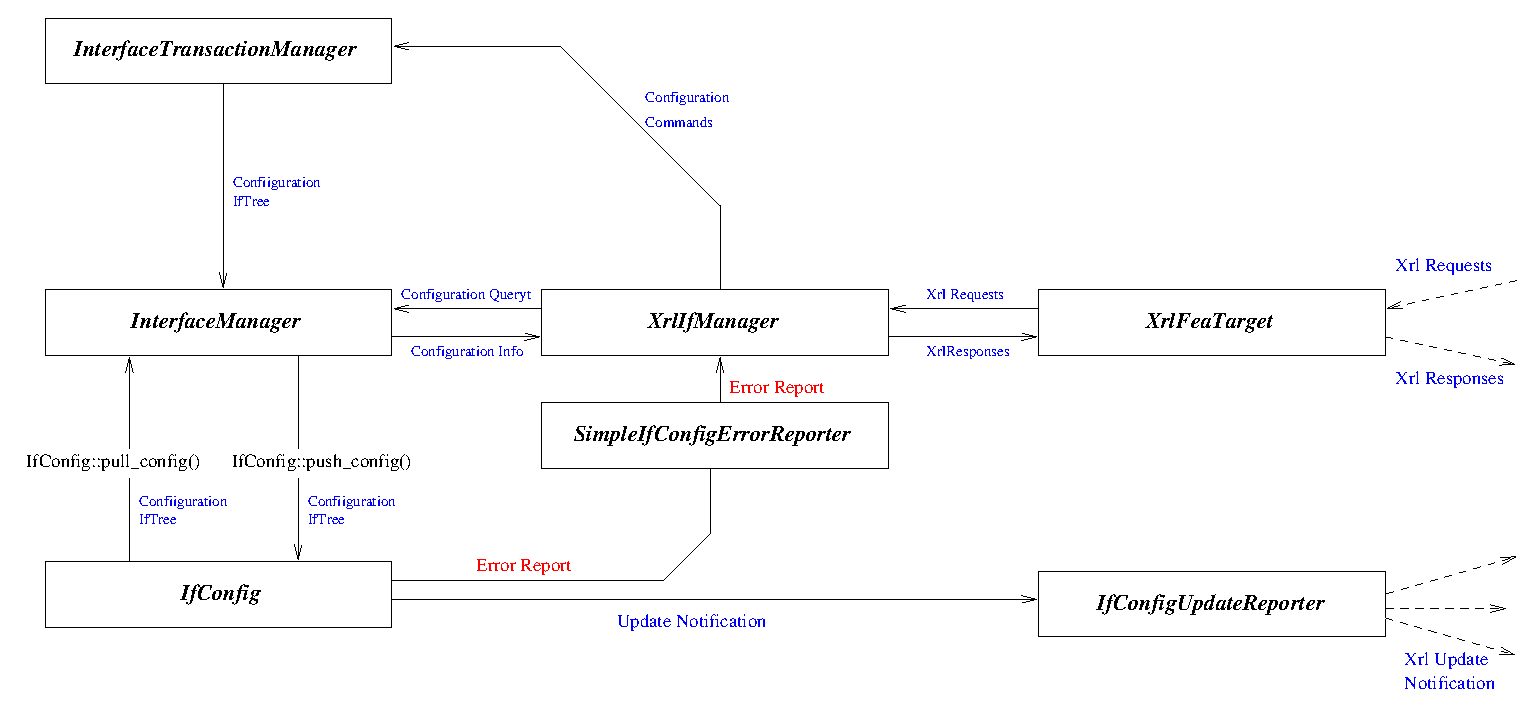
\includegraphics[angle=90,height=0.90\textheight]{figs/ifi}
    \caption{FEA Interface Management classes and their interactions}
    \label{fig:ifi}
  \end{center}
\end{figure}
\clearpage


%%%%%%%%%%%%%%%%%%%%%%%%%%%%%%%%%%%%%%%%%%%
\subsection{Forwarding Table Management}

The Forwarding Table Management role propagates routes into the
forwarding plane.  The Forwarding Table Management role does not
shadow the forwarding information outside of the forwarding plane
itself; rather, it relies on the RIB to do this.  As a result, it is
considerably simpler than the Interface Management role.

The classes interacting to provide the Forward Table Management role
are: the {\tt XrlFtiTransactionManager} class, a class that adapts
requests and responses from the subset of {\tt XrlFeaTarget} methods
that represent the forwarding table management externally; the {\tt
FtiTransactionManager} that builds and executes transactions to
configure the forwarding table; and class {\tt Fti} that understands
how to program the forwarding plane.

The {\tt Fti} class provides the interface for accessing the
forwarding plane.  It includes methods for adding and
removing routes, as well as resolving routes in the forwarding table.
Modifications to the {\tt Fti} state are only permitted during a
configuration interval.  The configuration interval is started and
stopped using {\tt Fti::start\_configuration} and {\tt
Fti:end\_configuration}.  The particular access to the forwarding
plane is performed by plug-ins that are specific to that
plane. For example, to read the forwarding table currently there are
plug-ins that utilize the sysctl(3) mechanism (\eg in case of FreeBSD)
or the netlink mechanism (\eg in case of Linux). There are
plug-ins to read, set or monitor the forwarding table information
at the granularity of one entry, or the whole table.

The {\tt FtiTransactionManager} presents a transactional interface for
configuring the {\tt Fti} instance.  Command classes exist for each
possible modifier operation on the {\tt Fti} instance.  The {\tt Fti}
methods {\tt start\_configuration} and {\tt end\_configuration} are
called at the start and end of the transaction.

%%%%%%%%%%%%%%%%%%%%%%%%%%%%%%%%%%%%%%%%%%%
\subsection{Interface Specific Packet I/O}

The Interface Specific Packet I/O role of the FEA provides a means for
XORP processes to send and receive packets on particular interfaces.
This is an essential function since in a XORP router the forwarding
plane may reside on a different machine to the routing processes, it
may be distributed across several machines, or may have custom network
interfaces that require special programming.  Currently (August 2003),
only the sending and receiving of raw IPv4 packets is implemented.
Support for UDP and IPv6 will follow in future and should follow a
similar design pattern to the raw IPv4 packet handling.

The raw packet interface is managed by the {\tt XrlRawSocket4Manager}
class.  This manages a single instance of a {\tt
FilterRawSocket4}\footnote{The current implementation only works on
single machine XORP forwarding planes}.  The {\tt FilterRawSocket4}
encapsulates a raw socket and allows raw IPv4 packets to be written
and filters attached to parse raw packets as they are received.  The
{\tt XrlRawSocket4Manager} allows an arbitrary number of filters to be
associated with the active raw socket.  The filters are each notified
when a raw packet is received on the raw socket.  The
XrlRawSocket4Manager allows other XORP processes to receive packets
via XRL on the basis on filter conditions.  Currently (August 2003),
the only implemented filter is the {\tt XrlVifInputFilter} which
allows processes to receive raw packets on the basis of the receiving
VIF.  In principle, filters could be written to match on any field
within a packet and perform an action.

%%%%%%%%%%%%%%%%%%%%%%%%%%%%%%%%%%%%%%%%%%%%%%%%%%%%%%%%%%%%%%%%%%%%%%%
\section{Status}
\label{sec:status}

Currently (August 2003), two versions of the FEA are supported: {\tt
fea} and {\tt fea\_dummy}.  The {\tt fea} is a version
of the FEA that contains plug-ins to access the forwarding plane by
using the following mechanisms:

\begin{itemize}

  \item {\it getifaddrs(3)}, {\it sysctl(3)}, {\it ioctl(3)},
   and {Linux /proc} to obtain interface-specific information.

  \item {\it ioctl(3)} to set interface-specific information.

  \item {\it routing sockets} for observing changes in the
  interface-specific information.

  \item {\it routing sockets} and {\it netlink sockets} to lookup
  a single forwarding entry in the forwarding plane.

  \item {\it sysctl(3)} and {\it netlink sockets} to obtain the whole
  forwarding table from the forwarding plane.

  \item {\it routing sockets} to set a single forwarding entry or the
  whole table in the forwarding plane.

  \item {\it routing sockets} to observe changes in the forwarding
  table.

\end{itemize}

In other words, currently (August 2003) the {\tt fea} supports FreeBSD for
reading and writing to the forwarding plane, and Linux for reading only (so
far it has been tested on FreeBSD-4.x and Linux-2.4.20).
The {\tt fea\_dummy} is a substitute FEA and may be
used for development testing purposes.  The {\tt fea\_dummy}
represents an idealized form of FEA, other FEA's may differ in their
responses due to architectural differences.  Therefore processes that
interact with the FEA should regard {\tt fea\_dummy} interactions as
indicative, but not definitive.

The FEA's are still a work in progress and no doubt have some bugs.
Any contributions or bug fixes are welcome.  Completing the FEA support
for Linix is work-in-progress. FEA support for Click is yet to
be written, and FEA's for any other architecture would
be welcomed.  There is a now defunct Click FEA in the {\tt \$XORP/fea}
directory that should be possible to resurrect.

%%%%%%%%%%%%%%%%%%%%%%%%%%%%%%%%%%%%%%%%%%%%%%%%%%%%%%%%%%%%%%%%%%%%%%%
%     BIBLIOGRAPHY
%%%%%%%%%%%%%%%%%%%%%%%%%%%%%%%%%%%%%%%%%%%%%%%%%%%%%%%%%%%%%%%%%%%%%%%
\bibliography{../tex/xorp}
\bibliographystyle{plain}

%%%%%%%%%%%%%%%%%%%%%%%%%%%%%%%%%%%%%%%%%%%%%%%%%%%%%%%%%%%%%%%%%%%%%%%
\end{document}
